%form: dc_form_03-04.tex ; user: dc_03-04_preparation_etc.tex
%========== DC =========
%===== p. 03-04 現在までの研究状況 =============
\section{現在までの研究状況}
%watermark: w03_past_dc
\newcommand{\研究の背景}{%
%begin  研究の背景===================
	\subsection{2.で述べた研究状況を踏まえこれからの研究計画の背景}
	\noindent
	●\textbf{2.で述べた研究状況を踏まえこれからの研究計画の背景}

	自然言語処理は、前後の文脈を考慮できるBERT\cite{devlin-etal-2019-bert}や前節で述べたGrover\cite{NIPS2019_9106}を始め、
	より自然な文章が近年は生成できるようになった。
	前節の研究では実際にGroverを拡張し\textbf{コメントを生成することでより多くのフェイクニュースを検出}した。
	今後は、より拡散を抑制できるモデルの開発を目指す。

	\subsection{問題点・解決すべき点}
	\noindent
	●\textbf{問題点・解決すべき点}

	生成コメントを付加して分類した場合、前節提案モデルがFakeと判断した中で実際にFakeだった割合である精度(Precision)は0.59だった。
	これは生成コメントを付加せず分類したときの0.68と比べ0.09ポイント下回る\cite{EasyChair:3190}。
	つまり多くのフェイクニュースを検出することができても、\textbf{41\%の確率で事実に基づくニュースもフェイクニュースと判定する狼少年のようなモデル}である。
	精度と再現率の調和平均であるF値(F1 score)も、提案モデルは\textbf{0.68}と単体で見ても決して高いものではなかった。
	同時に、生成されたコメントは文法面でのクオリティが決して良いものとは言えず、このままでは説明可能性に繋げることは難しい。
	これでは利用者の信用を得るのは難しく、拡散の抑制にはならない。

	この\textbf{分類性能改善}と、\textbf{不自然なコメントにより説明可能性を提供できない}2点を解決する必要がある。

	\subsection{着想に至った経緯}
	\noindent
	●\textbf{着想に至った経緯}

	実際に早期自動検出モデルをSNS上で運用する場合を想定した。
	このモデルの目的は拡散の抑制であるため、\textbf{フェイクニュース以上に利用者の信用を得なければ拡散を食い止められない}。
	そのためには、真偽分類の精度を上げることと、説得力向上のために説明可能性を同時に提供する必要があると考えた。

	{\small
		\begin{thebibliography}{99}
			\setcounter{enumiv}{5}
			\bibitem{devlin-etal-2019-bert} Jacob Devlin, \textit{et al.} BERT: Pre-training of deep bidirec-tional transformers for language understanding. In \textit{Proc. of the NAACL-HLT,} pp. 4171–4186, Minneapolis, Minnesota, June 2019.
		\end{thebibliography}
		%\bibliography{myreferences}
		%\bibliographystyle{junsrt}
	}
%end  研究の背景 ====================
}

\newcommand{\現在までの研究状況}{%
%begin  現在までの研究状況===================
	\subsection{これまでの研究の背景}
	\noindent
	●\textbf{これまでの研究の背景}

	SNSの発展により、情報を迅速に大量取得し、拡散することで容易に共有できるようになった。
	一方、悪意によって他人を騙すために作られた\textbf{フェイクニュース}が拡散されやすくなった。
	フェイクニュースが拡散されると、\textbf{誤った認識が広がって騙された人々が社会的損害を起こす}という問題がある。
	例えば、2016年米国大統領選挙前にフェイクニュースに騙された人々がピザ屋で銃撃事件を起こした\cite{agencies_2016}。
	また、今年は特にCOVID-19にまつわるフェイクニュースが広く拡散され、不安に陥った人々が買いだめを行うことが世界的に問題となった。
	WHOは情報の過剰な氾濫を``インフォデミック''と定義し、テドロス事務局長は\textbf{誤った情報はウイルス以上に拡散されやすい}と指摘した\cite{ZAROCOSTAS2020676}。

	\subsection{問題点}
	\noindent
	●\textbf{問題点}

	現在フェイクニュース対策として、有識者が事実関係の確認を行う\textbf{ファクトチェック}がとられている。
	ただしこれは\textbf{属人的な作業}であることに加え、拡散されてから調査されることが多く、結果を公表するまで時間がかかることからフェイクニュースと比べあまり\textbf{拡散されにくい}。
	これを自動で検出する場合、フェイクニュースは巧妙に実際のニュースを模した形をとるため、\textbf{単純なルールベース手法では難しい}。
	近年ではニューステキストや添付メディア、ユーザの反応から\textbf{ディープニューラルネットワーク(DNN)}を利用した手法がみられる。
	%この場合はブラックボックス問題により\textbf{説明可能性が不足}するため、SNS利用者から支持を得にくい。
	その中で\textbf{ユーザの反応は拡散後でしか得られない}ため、早期の発見を想定した場合はユーザの反応を評価対象にすることができない。

	\subsection{解決方策}
	\noindent
	●\textbf{解決方策}

	そこで本研究では\textbf{学習でのみユーザの反応を活用}し、テスト時は\textbf{ユーザの反応を生成・補完}して分類することで、
	\textbf{精度を落とさず早期発見を目指す}ことにした。

	\subsection{研究目的・研究方法}
	\noindent
	●\textbf{研究目的・研究方法}

	フェイクニュース早期発見に向け、SNS上で\textbf{ニュースに寄せられたコメントを生成する}ことが、
	\textbf{真偽を分類する精度の向上につながる}ことを示す。
	本研究はニュースと寄せられたコメントを、
	ニュースの本文と実際にSNS上で投稿されたコメント3件を1ユニットとして扱うことにした。
	
	\begin{figure}[ht]
		\centering
		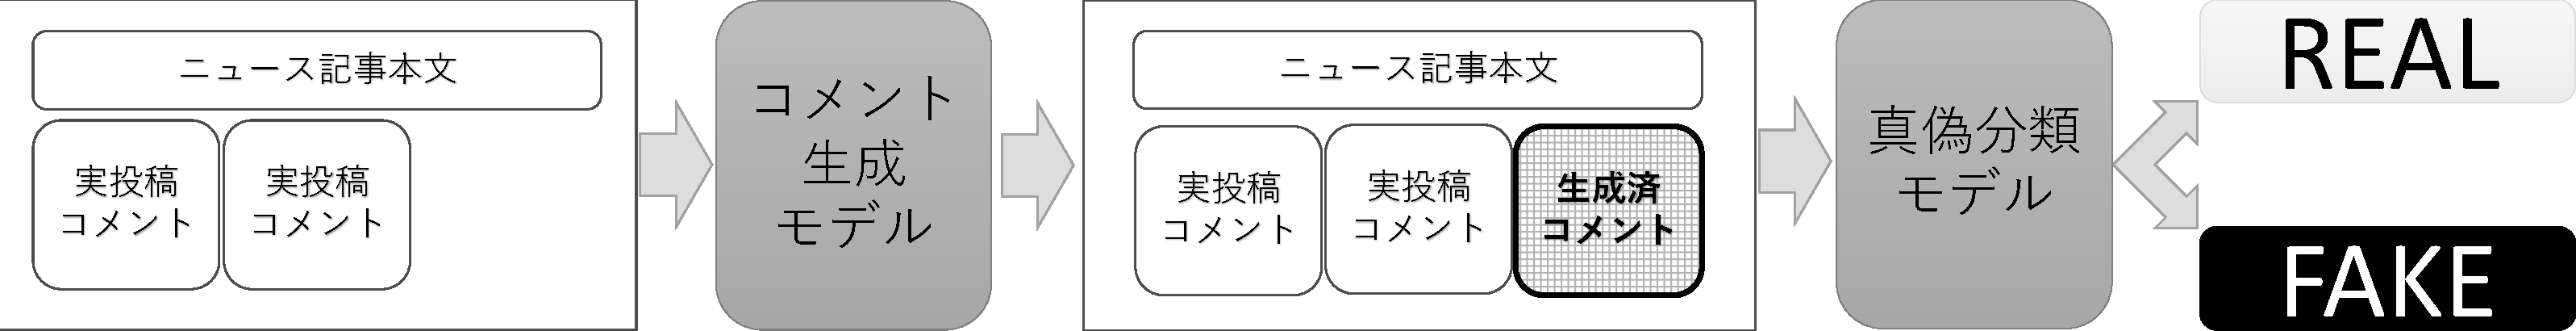
\includegraphics[width=0.95\linewidth]{figs/model.pdf}
		\caption{分類タスクの流れ。コメント生成モデルで1件コメントを生成し真偽分類に活用する。}
		\label{fig:model}
	\end{figure}

	\subsection{特色と独創的な点}
	\noindent
	●\textbf{特色と独創的な点}
	
	\begin{itemize}
		\item 生成タスクを分類タスクに役立てる点
		\item 分類性能を大きく失わずに速報性をもつことができる点
		\item 生成されたコメントは説明可能性に繋げることが可能である点
	\end{itemize}

	\subsection{これまでの研究経過及び得られた結果}
	\noindent
	●\textbf{これまでの研究経過及び得られた結果}

	申請者はデータセットとしてFakeNewsNet\cite{Shu2018FakeNewsNetAD}を使用した。
	このデータセットは、ファクトチェックで\textbf{真偽が評価済である英文ニュース}と、それに\textbf{Twitter上で言及された投稿(ツイート)}等をもつ。
	本研究では最低3件以上英文でコメントとしてツイートが寄せられた芸能ニュースを真偽で各2000件使用した。
	拡散の初期段階ではコメントの数は期待できないため、使用するコメントは各3件ずつ無作為に選出し、残りは対象から除外した。

	生成・分類モデルは、フェイクニュースを自動で作成するGroverモデル\cite{NIPS2019_9106}を拡張する形で実装した。
	このモデルはフェイクニュースをドメイン・著者・投稿日・見出し・本文の5要素に分け、\textbf{ランダムで歯抜けにして予測させる形で生成学習を実現}したものである。
	今回はこれをユニットの4要素(記事本文と3件のコメント)での実装を目指し調整を行った。
	訓練が完了したコメント生成モデルを使い、図\ref{fig:model}の通り\textbf{コメントを1件欠損させたユニットに生成コメントを付加した上で、RealかFakeか分類させた}。
	分類モデルはGroverが提供したものを流用した。

	その結果、生成コメントを含めた場合の\textbf{Fake記事を見抜いた割合を示す再現率(Recall)が0.79}と、欠損のまま分類させたときの\textbf{0.75}と、本文単独で分類したときの\textbf{0.62}を上回った。
	つまり、コメントを生成することで\textbf{ファクトチェックが必要な疑わしい記事をより多く検出}した\cite{EasyChair:3190}。
	同時に、生成されたコメントで頻出した単語の傾向において真偽で大きな違いはみられなかった。
	これは、\textbf{記事の真偽によってコメント内の単語傾向の差は軽微}であることを意味した。

	{\small 
	%\bibliography{myreferences}
	%\bibliographystyle{junsrt}
	\begin{thebibliography}{99}
		\bibitem{agencies_2016} Guardian staff and agencies. Washington gunman motivated by fake news `pizzagate' conspiracy,12 2016.
		\bibitem{ZAROCOSTAS2020676} John Zarocostas. How to fight an infodemic. \textit{The Lancet}, Vol. 395, No. 10225, p. 676, 2020.
		\bibitem{Shu2018FakeNewsNetAD} Kai Shu, \textit{et al.} Fakenewsnet: Adata repository with news content, social context and dynamic information for studying fake news on social media. \textit{ArXiv}, Vol. abs/1809.01286, 2018.
		\bibitem{NIPS2019_9106} Rowan Zellers, \textit{et al.} Defending against neural fake news. \textit{Advances in Neural Information Processing Systems 32}, pp. 9054–9065. Curran Associates, Inc., 2019.
		\bibitem{EasyChair:3190} Yuta Yanagi, \textit{et al.} Fake news detection with generated comments for news articles. \textit{EasyChair Preprint no. 3190}, EasyChair, 2020.
	\end{thebibliography}
	}
	%ぞうの卵はおいしいぞう。
ぞうの卵はおいしいぞう。
ぞうの卵はおいしいぞう。
ぞうの卵はおいしいぞう。
ぞうの卵はおいしいぞう。
ぞうの卵はおいしいぞう。
ぞうの卵はおいしいぞう。
ぞうの卵はおいしいぞう。
ぞうの卵はおいしいぞう。
ぞうの卵はおいしいぞう。
ぞうの卵はおいしいぞう。
ぞうの卵はおいしいぞう。
ぞうの卵はおいしいぞう。
ぞうの卵はおいしいぞう。
ぞうの卵はおいしいぞう。
ぞうの卵はおいしいぞう。
ぞうの卵はおいしいぞう。
ぞうの卵はおいしいぞう。
ぞうの卵はおいしいぞう。
ぞうの卵はおいしいぞう。
ぞうの卵はおいしいぞう。
ぞうの卵はおいしいぞう。
ぞうの卵はおいしいぞう。
ぞうの卵はおいしいぞう。
ぞうの卵はおいしいぞう。
ぞうの卵はおいしいぞう。
ぞうの卵はおいしいぞう。
ぞうの卵はおいしいぞう。
ぞうの卵はおいしいぞう。
ぞうの卵はおいしいぞう。
ぞうの卵はおいしいぞう。
ぞうの卵はおいしいぞう。
ぞうの卵はおいしいぞう。
ぞうの卵はおいしいぞう。
ぞうの卵はおいしいぞう。
ぞうの卵はおいしいぞう。
ぞうの卵はおいしいぞう。
ぞうの卵はおいしいぞう。
ぞうの卵はおいしいぞう。
ぞうの卵はおいしいぞう。
ぞうの卵はおいしいぞう。
ぞうの卵はおいしいぞう。
ぞうの卵はおいしいぞう。
ぞうの卵はおいしいぞう。
ぞうの卵はおいしいぞう。
ぞうの卵はおいしいぞう。
ぞうの卵はおいしいぞう。
ぞうの卵はおいしいぞう。
ぞうの卵はおいしいぞう。
ぞうの卵はおいしいぞう。
ぞうの卵はおいしいぞう。
ぞうの卵はおいしいぞう。
ぞうの卵はおいしいぞう。
ぞうの卵はおいしいぞう。
ぞうの卵はおいしいぞう。
ぞうの卵はおいしいぞう。
ぞうの卵はおいしいぞう。
ぞうの卵はおいしいぞう。
ぞうの卵はおいしいぞう。
ぞうの卵はおいしいぞう。
ぞうの卵はおいしいぞう。
ぞうの卵はおいしいぞう。
ぞうの卵はおいしいぞう。
ぞうの卵はおいしいぞう。
ぞうの卵はおいしいぞう。
ぞうの卵はおいしいぞう。
ぞうの卵はおいしいぞう。
ぞうの卵はおいしいぞう。
ぞうの卵はおいしいぞう。
ぞうの卵はおいしいぞう。
ぞうの卵はおいしいぞう。
ぞうの卵はおいしいぞう。
ぞうの卵はおいしいぞう。
ぞうの卵はおいしいぞう。
ぞうの卵はおいしいぞう。
ぞうの卵はおいしいぞう。
ぞうの卵はおいしいぞう。
ぞうの卵はおいしいぞう。
ぞうの卵はおいしいぞう。
ぞうの卵はおいしいぞう。
ぞうの卵はおいしいぞう。
ぞうの卵はおいしいぞう。
ぞうの卵はおいしいぞう。
ぞうの卵はおいしいぞう。
ぞうの卵はおいしいぞう。
ぞうの卵はおいしいぞう。
ぞうの卵はおいしいぞう。
ぞうの卵はおいしいぞう。
ぞうの卵はおいしいぞう。
ぞうの卵はおいしいぞう。
ぞうの卵はおいしいぞう。
ぞうの卵はおいしいぞう。
ぞうの卵はおいしいぞう。
ぞうの卵はおいしいぞう。
ぞうの卵はおいしいぞう。
ぞうの卵はおいしいぞう。
ぞうの卵はおいしいぞう。
ぞうの卵はおいしいぞう。
ぞうの卵はおいしいぞう。
ぞうの卵はおいしいぞう。
ぞうの卵はおいしいぞう。
ぞうの卵はおいしいぞう。
ぞうの卵はおいしいぞう。
ぞうの卵はおいしいぞう。
ぞうの卵はおいしいぞう。
ぞうの卵はおいしいぞう。
ぞうの卵はおいしいぞう。
ぞうの卵はおいしいぞう。
ぞうの卵はおいしいぞう。
ぞうの卵はおいしいぞう。
ぞうの卵はおいしいぞう。
ぞうの卵はおいしいぞう。
ぞうの卵はおいしいぞう。
ぞうの卵はおいしいぞう。
ぞうの卵はおいしいぞう。
ぞうの卵はおいしいぞう。
ぞうの卵はおいしいぞう。
ぞうの卵はおいしいぞう。
ぞうの卵はおいしいぞう。
ぞうの卵はおいしいぞう。
ぞうの卵はおいしいぞう。
ぞうの卵はおいしいぞう。
ぞうの卵はおいしいぞう。
ぞうの卵はおいしいぞう。
ぞうの卵はおいしいぞう。
ぞうの卵はおいしいぞう。
ぞうの卵はおいしいぞう。
ぞうの卵はおいしいぞう。
ぞうの卵はおいしいぞう。
ぞうの卵はおいしいぞう。
ぞうの卵はおいしいぞう。
ぞうの卵はおいしいぞう。
ぞうの卵はおいしいぞう。
ぞうの卵はおいしいぞう。
ぞうの卵はおいしいぞう。
ぞうの卵はおいしいぞう。
ぞうの卵はおいしいぞう。
ぞうの卵はおいしいぞう。
ぞうの卵はおいしいぞう。
ぞうの卵はおいしいぞう。
ぞうの卵はおいしいぞう。
ぞうの卵はおいしいぞう。
ぞうの卵はおいしいぞう。
ぞうの卵はおいしいぞう。
ぞうの卵はおいしいぞう。
ぞうの卵はおいしいぞう。
ぞうの卵はおいしいぞう。
ぞうの卵はおいしいぞう。
ぞうの卵はおいしいぞう。
ぞうの卵はおいしいぞう。
ぞうの卵はおいしいぞう。
ぞうの卵はおいしいぞう。
ぞうの卵はおいしいぞう。
ぞうの卵はおいしいぞう。
ぞうの卵はおいしいぞう。
ぞうの卵はおいしいぞう。
ぞうの卵はおいしいぞう。
  % << only for demonstration. Please delete it or comment it out.	
%end  現在までの研究状況 ====================
}

